\setcounter{equation}{0}
\chapter{Introduction}

Galaxies are key to understand our Universe. So far, human kind has been able to study in detail the closest ones. Distant galaxies are still challenging to detect. They contain however information of millions of stars and gas that could unravel mysteries like for example, how Milky Way type of galaxies formed. It is an open challenge to obtain as much information as possible from these young galaxies. One way to accomplish this is to look at their spectra. Astronomers noted that a that relevant fraction of these galaxies emitted a really strong line at a particular wavelength and named them Lyman Alpha Emitters (LAEs). The purpose of this monograph is to model and simulate LAEs in order to advance our knowledge about this galaxy population. \\

%Motivacion: As for motivation, these observations have a direct impact in studying the reionization epoch (\cite{review}), properties of the interstellar medium (ISM) and the intergalactic medium (IGM) (\cite{Behrens13}, \cite{DijkstraKramer}), constraining star formation rates of high redshift galaxies, understanding galaxy luminosity functions (\cite{Max}) and studying the large scale structure of the Universe. In all of these studies, an understanding of the processes that model the morphology and radiate transfer process behind the \lya line, is required. To fully understand the observed spectra of the LAEs, these galaxies must be modeled. \\

%Desglosar este primer parrafo

\section{The physics of Lyman Alpha Emitters}
\label{sec1:laes}
In the early Universe the most abundant elements were Hydrogen(H) and Helium(He), causing young galaxies to be rich in H atoms. Also, due to stellar activity in a galaxy, the surrounding gas can be ionized. These two facts leave the H atoms prone to excite and emit radiation at definite frequencies. One of these frequencies corresponds to the \lya line. \cite{PartridgePeebles}  \\

When a Hydrogen atom is excited, the only electron it has moves to a higher energy level. However after some time, it is no longer able to maintain itself in this state. For this, the electron goes back to the ground level. Finally, as the energy obtained from this de-excitement has to be conserved, it is emitted as a photon with a wavelength of 1215.67 $\AA$. This is the Lyman Alpha ( \lya) transition, discovered by Theodore Lyman in 1906. \cite{LymanBio} \\

\lya radiation is emitted from the H atoms in a galaxy. Due to the amount of atoms inside it, the whole body could become a strong \lya radiator. Astronomers can take spectra of a galaxy to detect emission at that wavelength. If the galaxy shows a strong \lya line, it classifies as a Lyman Alpha Emitter (LAE). (\cite{DjorgovskiThompson}, \cite{Rhoads00}, \cite{Gawiser2007}, \cite{Koehler2007}, \cite{Ouchi08}, \cite{Yamada2012}, \cite{Schenker2012}, \cite{Kulas12}, \cite{Yamada2012}, \cite{Chonis2013}, \cite{Finkelstein2013}, \cite{Ostlin14}, \cite{Hayes2014}, \cite{Faisst2014}, \cite{Fumagalli2015}) \\

%However, the line is not a single peak at 1215.67 $\AA$ as one would first expect, but it strews around this wavelength in a particular shape. This morphology depends mostly on the galaxy's dynamics, chemistry and thermodynamics.\\

\begin{figure}[h!]
	\begin{center}
		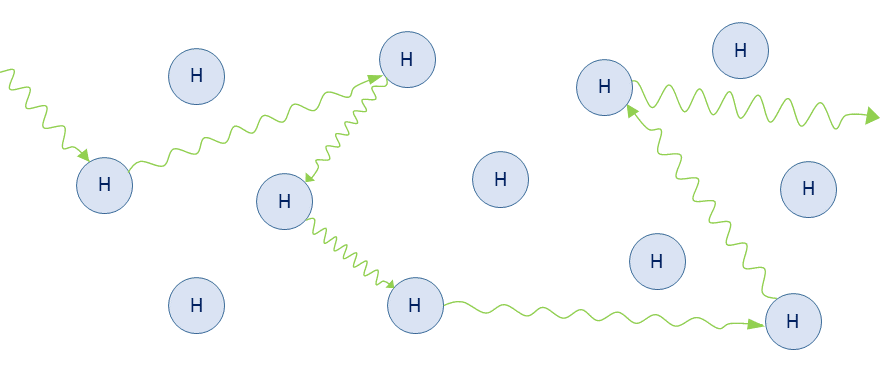
\includegraphics[width=1\textwidth]{./figures/chapter1/radiative_transfer}
	\end{center}
	\caption{\textbf{Radiative Transfer Sketch:} A \lya photon being absorbed and re-emitted by Hydrogen atoms. 
		\label{fig:radiative_transfer}}
\end{figure}

When a \lya photon is emitted inside the galaxy, it travels through its interstellar medium (ISM). During the photon's path it can be absorbed and re-emitted by an H atom. The new frequency of the photon is different that the initial one, in an observer frame of reference due to the atom's velocity. In LAEs, the state of the ISM gas, before and after a photon's re-emission is pretty much the same. This allows a random walk approximation and consider photon-atom encounters as scatterings. A photon's scattering can happen several times, as seen in Fig. \ref{fig:radiative_transfer}. This stops only until the photon is able to escape the galaxy. \\

\begin{figure}[h!]
	\begin{center}
		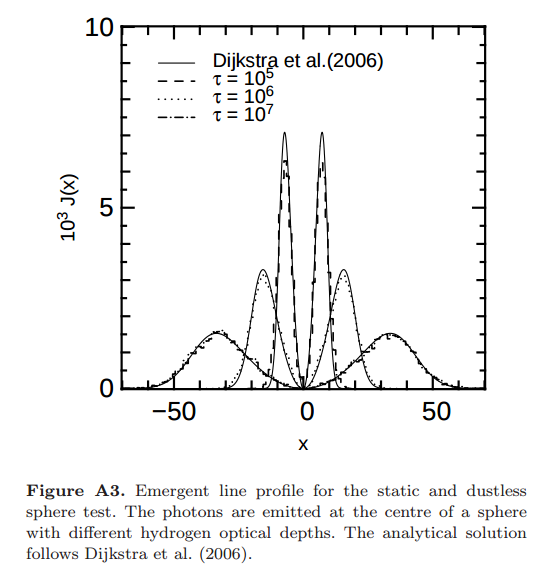
\includegraphics[width=0.6\textwidth]{./figures/chapter1/static}
	\end{center}
	\caption{\textbf{Figure A3 of Forero-Romero et al. paper:} CLARA's view on the escape fraction of Lyman-$\alpha$ photons in high redshift galaxies \cite{CLARA}. Reproduced with the permission of the author.
		\label{fig:static}}
\end{figure}

In a static galaxy, this random walk process produces a spectrum with two equal and symmetric peaks around the natural \lya wavelength. This can be seen in Figure A3 of Forero-Romero et al. paper \cite{CLARA} (Fig. \ref{fig:static}). If now the gas has a bulk velocity, the shape of the \lya profile changes. I explore these effects in this work by proposing a new model for a LAE. It consists of an spherical distribution of H atoms undergoing a solid body rotation and radial expansion(outflows). This new model can help observers to determine physical characteristics of a LAE by just looking at its \lya line. \\

The main goal is to measure the effect of the model's physical parameters on the outgoing \lya line. In this case, due to the resonant nature of the \lya line, analytical solutions can not be derived. It becomes necessary to run simulations to explore and test the model. \\

In this monograph I use a radiative transfer code that exists in the literature called CLARA (Code for Lyman Alpha Radiation Analysis). CLARA was written by Forero-Romero et al. \cite{CLARA}. It can simulate the \lya line of a spherical rotating LAE depending on its mass and velocity. In this work I modify CLARA to include outflows and explore the resulting consequences on the \lya line. \\